\documentclass[journal, a4paper]{IEEEtran}

%\usepackage{cite}
\usepackage{graphicx}
%\usepackage{psfrag}
%\usepackage{subfigure}
\usepackage{url}
%\usepackage{stfloats}
\usepackage{amsmath}
%\usepackage{array}
\usepackage{gensymb}

% Package Settings
\graphicspath{ {../images/} }

\begin{document}

% Define document title and author
\title{Testing the Effects of Transfection on Mammalian Cytokine RNA Expression}
\author{Austin Mitchell Vecchio
\thanks{Advisor: Dipl.--Ing.~Michelle Ammerman, Lehrstuhl f\"ur Nachrichtentechnik, TUM, WS 2050/2051.}}
\markboth{Hauptseminar Digitale Kommunikationssysteme}{}
\maketitle

% Write abstract here
\begin{abstract}
  Abstract outline

  This experiment aims to study the effect of genetic expression on polyplex treated cells against $\beta$-actin and INF$\alpha$.

\end{abstract}

% Each section begins with a \section{title} command
\section{Introduction}
    \PARstart{T}{his} section introduces the topic and leads the reader on to the main part.

Reverse Transcriptase (RT)qPCR is a technique used to describe the level of genetic expression is occuring in vitro
by measuring the amount of mRNA within a sample. In this technique, mRNA is reverse transcribed in to complementary DNA by
an enzyme labeled reverse transcriptase.

In this experiment, $\beta$-actin and RPL13A will be used for direct controls against the immunological transcripts.
INF$\beta$ will not be used as it will only appear after cycle 40 in the experiment producing undesirable results.
The No Template Control will consist of DEPC water.

Interleukin-6 (IL-6) is a multifunctional cytokine that defends the host in response
to immune and hematopoietic activities.

%Beta actin is an actin isoform that is highly involved in cell motility, structure and integrity.

%Beta-actin (human gene and protein symbol ACTB/ACTB) is one of six different actin isoforms which have been identified in humans. This is one of the two nonmuscle cytoskeletal actins. Actins are highly conserved proteins that are involved in cell motility, structure and integrity.

%Qubit

%http://www.ncbi.nlm.nih.gov/pmc/articles/PMC2143693/pdf/9144766.pdf
%http://www.molbiolcell.org/content/22/21/4047.full.pdf+html?with-ds=yes

For the QtPCR, since it is impossible to eliminate all genomic DNA from the cDNA synthesis, two solutions will be prepared. The first solution will be a +RT which will include reverse transcriptase and thus, will have cDNA.
The second solution will be a -RT solution which will lack reverse transcriptase. When QtPCR is performed on the -RT solution, genomic DNA will be amplified and will be seen in the resulting data.

\section{Methods}
    \subsection{RNA Purification}
      The cells in trizol were thawed before phase separation. During phase separation,
      the poly treated cells in trizol were incubated after which an addition of chloroform was added.
      The homoginized sample was incubated following a vigorous shake. The sample was then centrifuged before transfering the aqueous phase
      to a second tube. Isopropanol was added to the aqueous phase. The solution underwent a series of centrifuges in between removing ethanol
      resulting in an RNA pellet. The pellet was incubated following a resuspension in RNase free water.

    \subsection{cDNA Synthesis}
      For the first step of cDNA Synthesis, two solutions (+RT/-RT) were formed from the following compounds:
      10x dsDNase Buffer, dsDNase, Template RNA, polyplex 24hour RNA and nuclease free water.
      Both solutions were incubated after being centrifuged. The solutions were then chilled on ice, centrifuged and placed back on ice.
      For both solutions, 5X Reaction mix and nuclease free water was added. In the +RT solution, Maxima Enzyme mix (reverse transcriptase) was added to the mixture.
      The -RT solution used DEPC H20 instead of Maxima Enzyme mix so that the -RT solution can simulate the +RT solution without synthesizing RNA into cDNA.
      When the -RT solution undergoes QtPCR, any contaminating genomic DNA will be amplified.
      The two solutions will be then mixed gently and centrifuged. An incubation period will take place at 25$^{\circ}$C for 10 min
      followed by a second incubation session at 50$^{\circ}$C for 15 min.
      The reaction will be terminated by heating the solutions at 85$^{\circ}$C for 5 min.
      This process was conducted using Maxima First Strand cDNA Synthesis Kit with dsDNase (Thermo Scientific, Cat#: K1671)

    \subsection{Qt PCR}
      Each well will contain 2X iTaq universal SYBR Green Supermix,
      one of the four primers (IL6, INF$\alpha$, $\beta$-actin or RPL13A),
      and the respective cDNA.
      The cDNA needs to be diluted to 100ng/$\mu$L before it is added to the wells.
      The concentrations of cDNA for both sets of Poly24 and no washed cells were all around 100ng/ $\mu$ L.
      Therefore only one set of calculations were needed for determining the proper dilution of cDNA into water
      for either INF$\alpha$ and IL6 or $\beta$-actin andRPL13A and the respective -RT wells. For just cells,
      a different set of calculations were needed since the original cDNA concentrations were around 11 ng/ $\mu$ L.
      All wells contained the Green Supermix. The columns were sorted in the following manner:
      1-3 contained IL6, 4-6 contained INF$\alpha$, 7-9 contained $\beta$-acting and 10-12 contained RPL13A.
      The QtPCR was ran for 40 cycles.

    \subsection{Gel Electrophoresis}
      In order to further understand the results gained from the QtPCR, an agarose gel was ran.
      The wells were constructed in the following manner:
      (1) Ladder, (2) E1, (3) E3, (4) G1, (5) E2, (6) B1, (7) C1,
      (8) A5, (9) C4, (10) A8, (11) D10, (12) E11, (13) E12, (14) A8, (15) Ladder

    \subsection{Analysis}
      The results from the QtPCR produced Ct values from each well.
      A Ct value is a numeric inverse correlation to the quantity of nucleic acid detected by the aparatus.
      The Ct values can be used in combination with the $\Delta$\Delta$ct formula to produce fold inductions.

\section{Results}

  \subsection{Qubit}
    \begin{table}[!hbt]
      % Center the table
      \begin{center}
      % Fold Inductions
      \caption{Qubit Results}
      \label{tab:simParameters}
      % Table itself: here we have two columns which are centered and have lines to the left, right and in the middle: |c|c|
      \begin{tabular}{|c|c|}
      \hline
      SD1 & 54.27 \\
      \hline
      SD2 & 1057.52 \\
      \hline
      Tk & 8.75 \\
      \hline
      DA & 68.0 \\
      \hline
      AV & 487.0 \\
      \hline
      Tk & 28.0 \\
      \hline
      \end{tabular}
      \end{center}
    \end{table}

  \subsection{QtPCR}

  \subsection{Gel Electrophoresis}

\section{Discussion}

For a future experiment, it would be suggested that the polyplex cells are treated in 3 hour increments from 3 hours to 24 hours.

\section{Conclusion}
The mRNA was purified and converted to cDNA. THe resulting concentration was relatively high compared to peers. This eludes that the
treatment for these cells of polycationic DNA for 24 hours could result in higher transcription rates.

\section{Figures}

  \begin{figure}[t]
    \centering
    \caption{Agarose Gel}
    \label{fig:mesh1}
  \end{figure}

  \begin{table}[!hbt]
    % Center the table
    \begin{center}
    % Fold Inductions
    \caption{Wells for Immunological Responses}
    \label{tab:simParameters}
    % Table itself: here we have two columns which are centered and have lines to the left, right and in the middle: |c|c|
    \begin{tabular}{|c|c|c|c|c|c|c|c|c|c|c|c|c|}
      \hline
      & 1 & 2 & 3 & 4 & 5 & 6\\
      \hline
      A & 4ng/$\mu$L & 4ng/$\mu$L & 4ng/$\mu$L & 4ng/$\mu$L & 4ng/$\mu$L & 4ng/$\mu$L\\
      \hline
      B & 4ng/$\mu$L & 4ng/$\mu$L & 4ng/$\mu$L & 4ng/$\mu$L & 4ng/$\mu$L & 4ng/$\mu$L\\
      \hline
      C & 4ng/$\mu$L & 4ng/$\mu$L & 4ng/$\mu$L & 4ng/$\mu$L & 4ng/$\mu$L & 4ng/$\mu$L\\
      \hline
      D & 4ng/$\mu$L & 4ng/$\mu$L & 4ng/$\mu$L & 4ng/$\mu$L & 4ng/$\mu$L & 4ng/$\mu$L\\
      \hline
      E & Ts & Ni & AV & Ts & Ni & AV\\
      \hline
      E & Ts & Ni & AV & Ts & Ni & AV\\
      \hline
      G & Mi -RT & Mi NTC & & Mi -RT & Mi NTC & \\
      \hline
      H & & & & & &\\
      \hline
    \end{tabular}
    \end{center}
  \end{table}

  \begin{table}[!hbt]
    % Center the table
    \begin{center}
    % Fold Inductions
    \caption{Wells for Controls}
    \label{tab:simParameters}
    % Table itself: here we have two columns which are centered and have lines to the left, right and in the middle: |c|c|
    \begin{tabular}{|c|c|c|c|c|c|c|c|c|c|c|c|c|}
      \hline
      & 7 & 8 & 9 & 10 & 11 & 12 \\
      \hline
      A & 4ng/$\mu$L & 4ng/$\mu$L & 4ng/$\mu$L & 4ng/$\mu$L & 4ng/$\mu$L & 4ng/$\mu$L\\
      \hline
      B & 4ng/$\mu$L & 4ng/$\mu$L & 4ng/$\mu$L & 4ng/$\mu$L & 4ng/$\mu$L & 4ng/$\mu$L\\
      \hline
      C & 4ng/$\mu$L & 4ng/$\mu$L & 4ng/$\mu$L & 4ng/$\mu$L & 4ng/$\mu$L & 4ng/$\mu$L\\
      \hline
      D & 4ng/$\mu$L & 4ng/$\mu$L & 4ng/$\mu$L & 4ng/$\mu$L & 4ng/$\mu$L & 4ng/$\mu$L\\
      \hline
      E & Ts & Ni & AV & Ts & Ni & AV\\
      \hline
      E & Ts & Ni & AV & Ts & Ni & AV\\
      \hline
      G & Mi -RT & Mi NTC & & Mi -RT & Mi NTC & \\
      \hline
      H & & & & & &\\
      \hline
    \end{tabular}
    \end{center}
  \end{table}

  \begin{figure}[t]
    \centering
    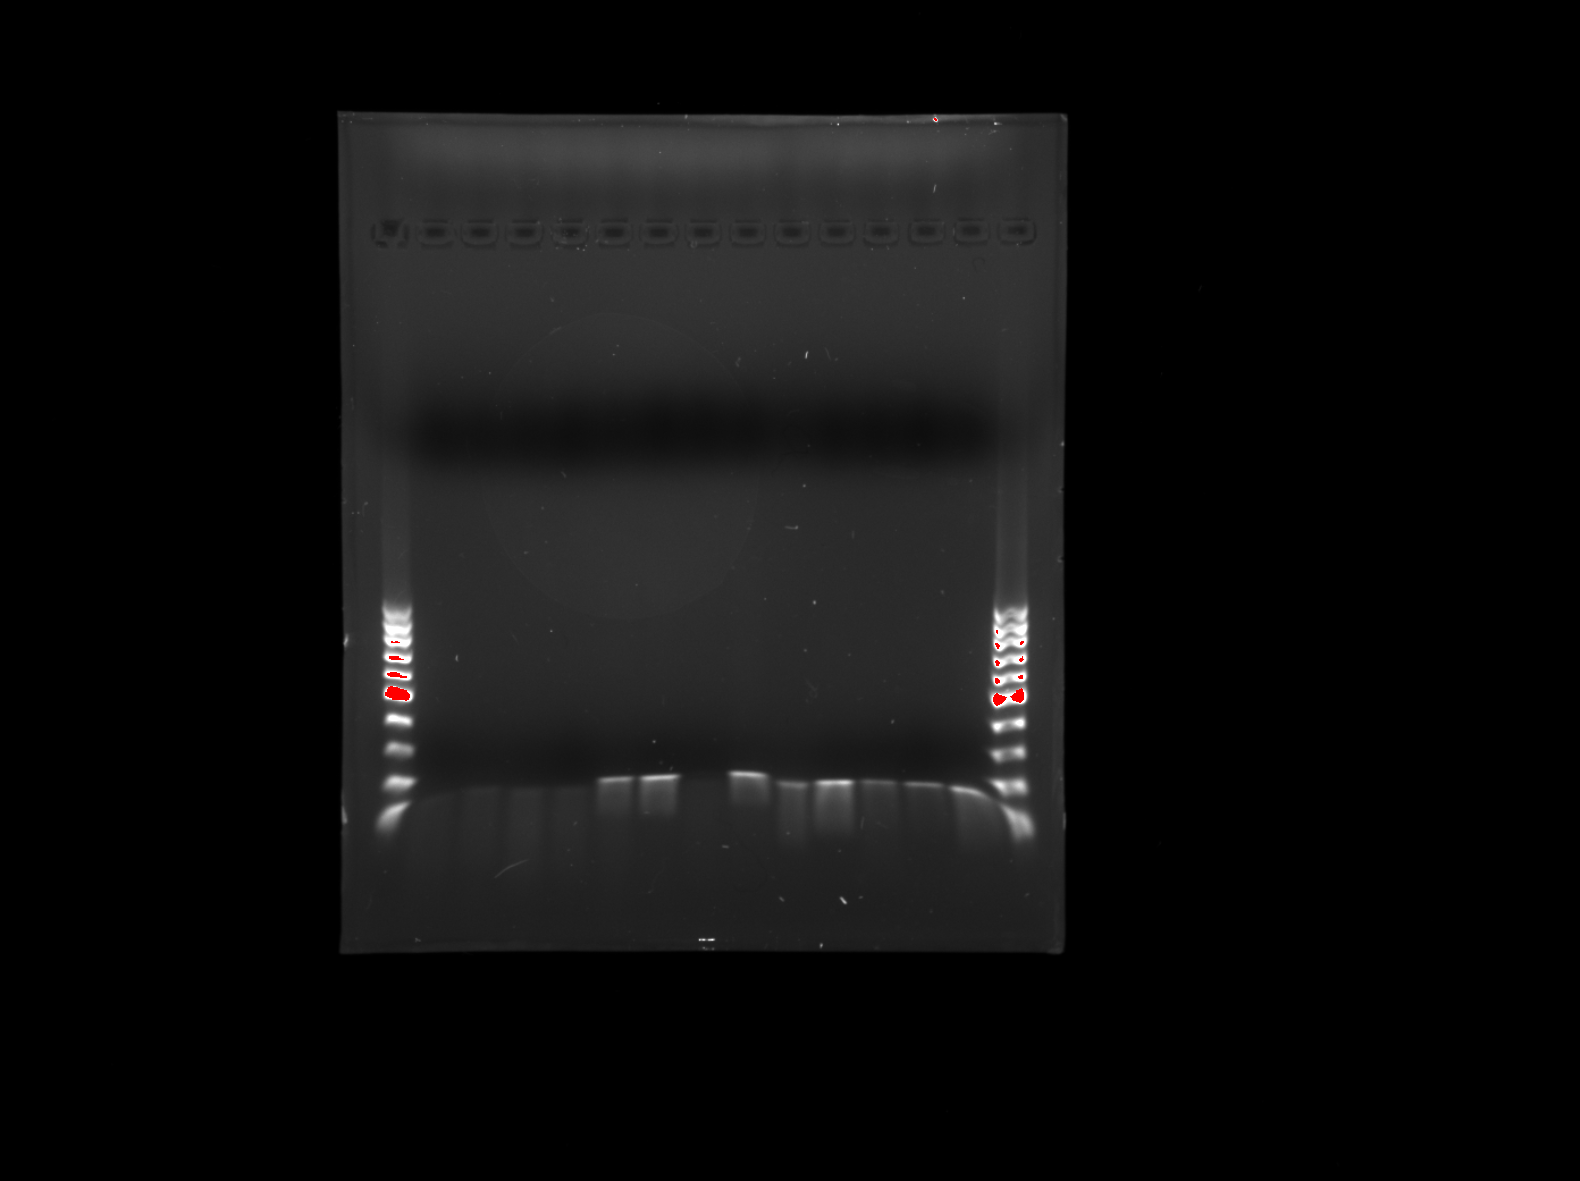
\includegraphics[width=8cm]{gel}
    \caption{Agarose Gel}
    \label{fig:mesh1}
  \end{figure}

  \begin{figure}[t]
    \centering
    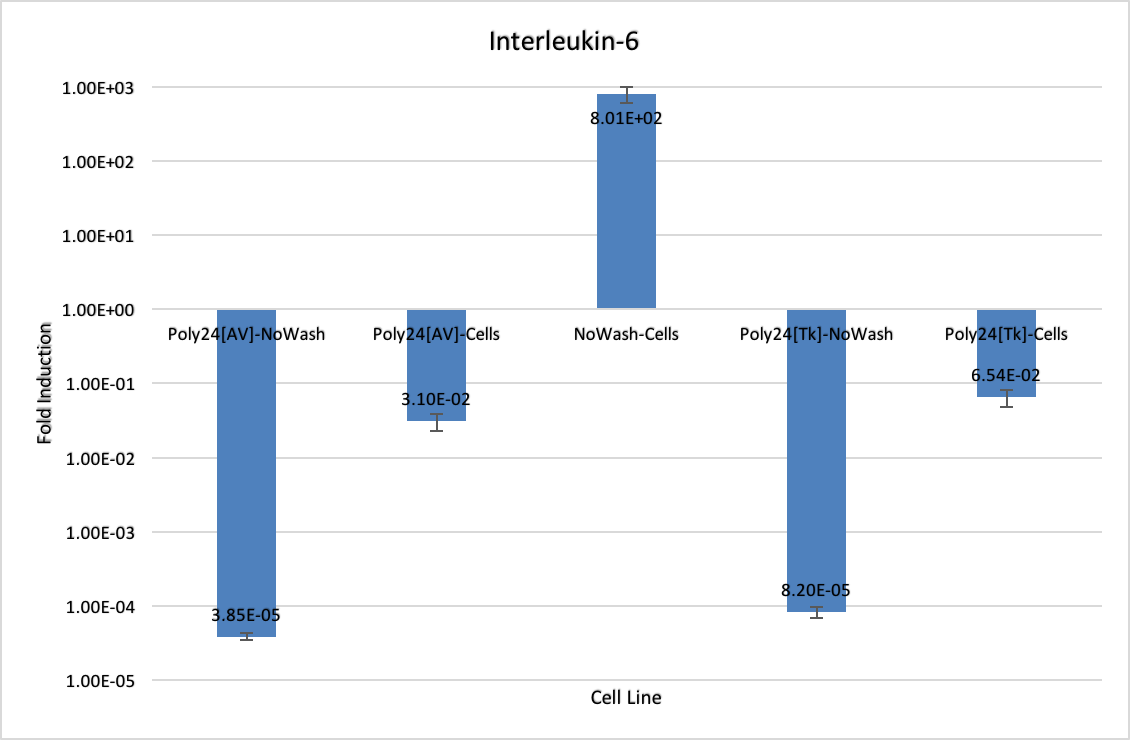
\includegraphics[width=8cm]{il6}
    \caption{Fold Inductions for}
    \label{fig:mesh1}
  \end{figure}

  \begin{figure}[t]
    \centering
    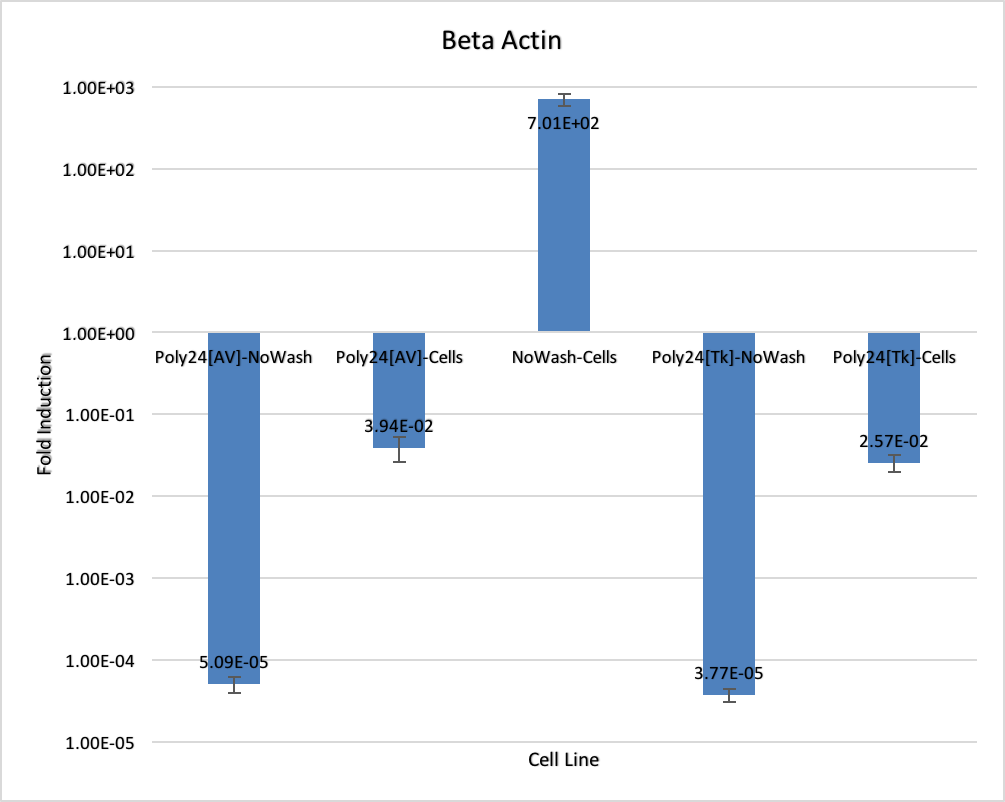
\includegraphics[width=8cm]{bactin}
    \caption{Fold Inductions for}
    \label{fig:mesh1}
  \end{figure}

  \begin{figure}[t]
    \centering
    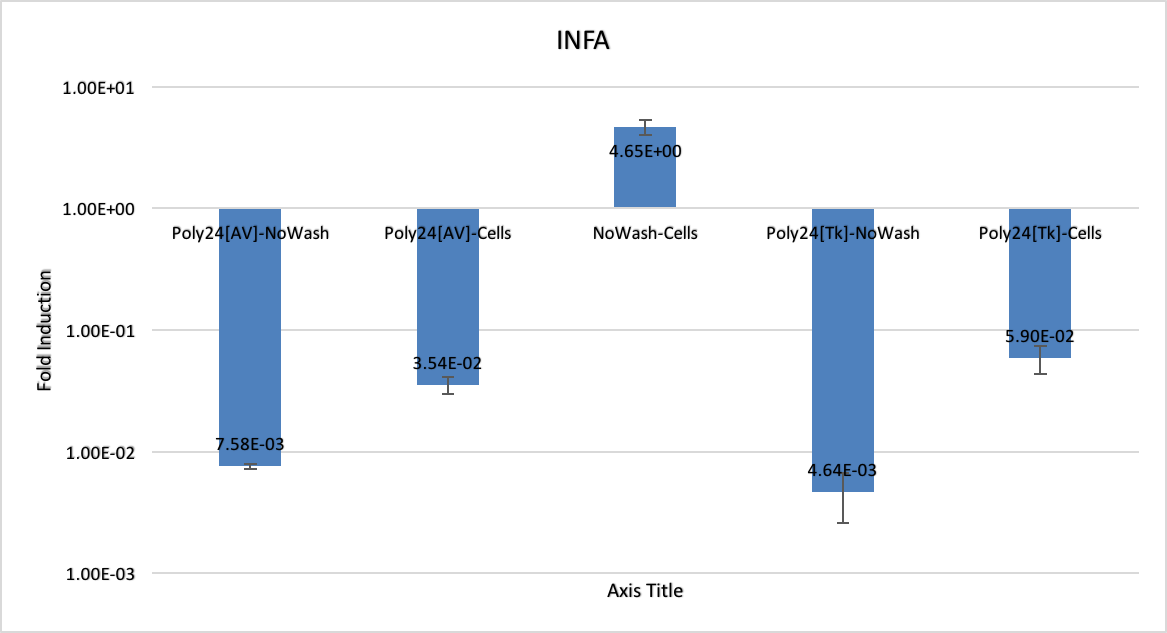
\includegraphics[width=8cm]{infa}
    \caption{Fold Inductions for}
    \label{fig:mesh1}
  \end{figure}

  \begin{figure}[t]
    \centering
    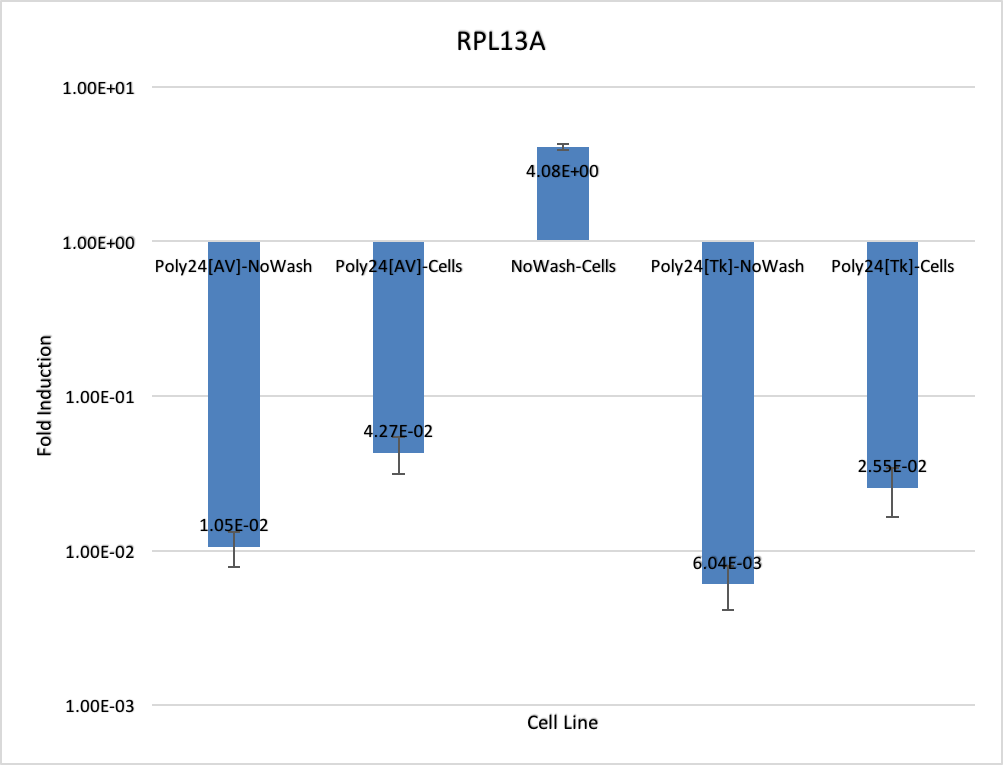
\includegraphics[width=8cm]{rpl13a}
    \caption{Fold Inductions for}
    \label{fig:mesh1}
  \end{figure}

% Now we need a bibliography:
\begin{thebibliography}{5}
    %Each item starts with a \bibitem{reference} command and the details thereafter.
    \bibitem{HOP96} % Transaction paper
    J.~Hagenauer, E.~Offer, and L.~Papke. Iterative decoding of binary block
    and convolutional codes. {\em IEEE Trans. Inform. Theory},
    vol.~42, no.~2, pp.~429–-445, Mar. 1996.

    \bibitem{MJH06} % Conference paper
    T.~Mayer, H.~Jenkac, and J.~Hagenauer. Turbo base-station cooperation for intercell interference cancellation. {\em IEEE Int. Conf. Commun. (ICC)}, Istanbul, Turkey, pp.~356--361, June 2006.

    \bibitem{Proakis} % Book
    J.~G.~Proakis. {\em Digital Communications}. McGraw-Hill Book Co.,
    New York, USA, 3rd edition, 1995.

    \bibitem{talk} % Web document
    F.~R.~Kschischang. Giving a talk: Guidelines for the Preparation and Presentation of Technical Seminars.
    \url{http://www.comm.toronto.edu/frank/guide/guide.pdf}.

    \bibitem{5}
    IEEE Transactions \LaTeX and Microsoft Word Style Files.
    \url{http://www.ieee.org/web/publications/authors/transjnl/index.html}

%    @Article{Gabay2006,
%    author="Gabay, Cem",
%    title="Interleukin-6 and chronic inflammation",
%    journal="Arthritis Research {\&} Therapy",
%    year="2006",
%    volume="8",
%    number="2",
%    pages="1--6",
%    abstract="Interleukin (IL)-6 is produced at the site of inflammation and plays a key role in the acute phase response as defined by a variety of clinical and biological features such as the production of acute phase proteins. IL-6 in combination with its soluble receptor sIL-6R$\alpha$, dictates the transition from acute to chonic inflammation by changing the nature of leucocyte infiltrate (from polymorphonuclear neutrophils to monocyte/macrophages). In addition, IL-6 exerts stimulatory effects on T- and B-cells, thus favoring chronic inflammatory responses. Strategies targeting IL-6 and IL-6 signaling led to effective prevention and treatment of models of rheumatoid arthritis and other chronic inflammatory diseases.",
%    issn="1478-6354",
%    doi="10.1186/ar1917",
%    url="http://dx.doi.org/10.1186/ar1917"
%    }

\end{thebibliography}

% Your document ends here!
\end{document}
